% Options for packages loaded elsewhere
\PassOptionsToPackage{unicode}{hyperref}
\PassOptionsToPackage{hyphens}{url}
\PassOptionsToPackage{dvipsnames,svgnames,x11names}{xcolor}
%
\documentclass[
  letterpaper,
  DIV=11,
  numbers=noendperiod]{scrreprt}
\usepackage{amsmath,amssymb}
\usepackage{lmodern}
\usepackage{iftex}
\ifPDFTeX
  \usepackage[T1]{fontenc}
  \usepackage[utf8]{inputenc}
  \usepackage{textcomp} % provide euro and other symbols
\else % if luatex or xetex
  \usepackage{unicode-math}
  \defaultfontfeatures{Scale=MatchLowercase}
  \defaultfontfeatures[\rmfamily]{Ligatures=TeX,Scale=1}
\fi
% Use upquote if available, for straight quotes in verbatim environments
\IfFileExists{upquote.sty}{\usepackage{upquote}}{}
\IfFileExists{microtype.sty}{% use microtype if available
  \usepackage[]{microtype}
  \UseMicrotypeSet[protrusion]{basicmath} % disable protrusion for tt fonts
}{}
\makeatletter
\@ifundefined{KOMAClassName}{% if non-KOMA class
  \IfFileExists{parskip.sty}{%
    \usepackage{parskip}
  }{% else
    \setlength{\parindent}{0pt}
    \setlength{\parskip}{6pt plus 2pt minus 1pt}}
}{% if KOMA class
  \KOMAoptions{parskip=half}}
\makeatother
\usepackage{xcolor}
\setlength{\emergencystretch}{3em} % prevent overfull lines
\setcounter{secnumdepth}{5}
% Make \paragraph and \subparagraph free-standing
\ifx\paragraph\undefined\else
  \let\oldparagraph\paragraph
  \renewcommand{\paragraph}[1]{\oldparagraph{#1}\mbox{}}
\fi
\ifx\subparagraph\undefined\else
  \let\oldsubparagraph\subparagraph
  \renewcommand{\subparagraph}[1]{\oldsubparagraph{#1}\mbox{}}
\fi


\providecommand{\tightlist}{%
  \setlength{\itemsep}{0pt}\setlength{\parskip}{0pt}}\usepackage{longtable,booktabs,array}
\usepackage{calc} % for calculating minipage widths
% Correct order of tables after \paragraph or \subparagraph
\usepackage{etoolbox}
\makeatletter
\patchcmd\longtable{\par}{\if@noskipsec\mbox{}\fi\par}{}{}
\makeatother
% Allow footnotes in longtable head/foot
\IfFileExists{footnotehyper.sty}{\usepackage{footnotehyper}}{\usepackage{footnote}}
\makesavenoteenv{longtable}
\usepackage{graphicx}
\makeatletter
\def\maxwidth{\ifdim\Gin@nat@width>\linewidth\linewidth\else\Gin@nat@width\fi}
\def\maxheight{\ifdim\Gin@nat@height>\textheight\textheight\else\Gin@nat@height\fi}
\makeatother
% Scale images if necessary, so that they will not overflow the page
% margins by default, and it is still possible to overwrite the defaults
% using explicit options in \includegraphics[width, height, ...]{}
\setkeys{Gin}{width=\maxwidth,height=\maxheight,keepaspectratio}
% Set default figure placement to htbp
\makeatletter
\def\fps@figure{htbp}
\makeatother
\newlength{\cslhangindent}
\setlength{\cslhangindent}{1.5em}
\newlength{\csllabelwidth}
\setlength{\csllabelwidth}{3em}
\newlength{\cslentryspacingunit} % times entry-spacing
\setlength{\cslentryspacingunit}{\parskip}
\newenvironment{CSLReferences}[2] % #1 hanging-ident, #2 entry spacing
 {% don't indent paragraphs
  \setlength{\parindent}{0pt}
  % turn on hanging indent if param 1 is 1
  \ifodd #1
  \let\oldpar\par
  \def\par{\hangindent=\cslhangindent\oldpar}
  \fi
  % set entry spacing
  \setlength{\parskip}{#2\cslentryspacingunit}
 }%
 {}
\usepackage{calc}
\newcommand{\CSLBlock}[1]{#1\hfill\break}
\newcommand{\CSLLeftMargin}[1]{\parbox[t]{\csllabelwidth}{#1}}
\newcommand{\CSLRightInline}[1]{\parbox[t]{\linewidth - \csllabelwidth}{#1}\break}
\newcommand{\CSLIndent}[1]{\hspace{\cslhangindent}#1}

% Soul package to handle highlighting (see hl.py3 filter)
\usepackage{soul}
\KOMAoption{captions}{tableheading}
\makeatletter
\@ifpackageloaded{tcolorbox}{}{\usepackage[many]{tcolorbox}}
\@ifpackageloaded{fontawesome5}{}{\usepackage{fontawesome5}}
\definecolor{quarto-callout-color}{HTML}{909090}
\definecolor{quarto-callout-note-color}{HTML}{0758E5}
\definecolor{quarto-callout-important-color}{HTML}{CC1914}
\definecolor{quarto-callout-warning-color}{HTML}{EB9113}
\definecolor{quarto-callout-tip-color}{HTML}{00A047}
\definecolor{quarto-callout-caution-color}{HTML}{FC5300}
\definecolor{quarto-callout-color-frame}{HTML}{acacac}
\definecolor{quarto-callout-note-color-frame}{HTML}{4582ec}
\definecolor{quarto-callout-important-color-frame}{HTML}{d9534f}
\definecolor{quarto-callout-warning-color-frame}{HTML}{f0ad4e}
\definecolor{quarto-callout-tip-color-frame}{HTML}{02b875}
\definecolor{quarto-callout-caution-color-frame}{HTML}{fd7e14}
\makeatother
\makeatletter
\makeatother
\makeatletter
\@ifpackageloaded{caption}{}{\usepackage{caption}}
\AtBeginDocument{%
\ifdefined\contentsname
  \renewcommand*\contentsname{Índice}
\else
  \newcommand\contentsname{Índice}
\fi
\ifdefined\listfigurename
  \renewcommand*\listfigurename{Lista de Figuras}
\else
  \newcommand\listfigurename{Lista de Figuras}
\fi
\ifdefined\listtablename
  \renewcommand*\listtablename{Lista de Tabelas}
\else
  \newcommand\listtablename{Lista de Tabelas}
\fi
\ifdefined\figurename
  \renewcommand*\figurename{Figura}
\else
  \newcommand\figurename{Figura}
\fi
\ifdefined\tablename
  \renewcommand*\tablename{Tabela}
\else
  \newcommand\tablename{Tabela}
\fi
}
\@ifpackageloaded{float}{}{\usepackage{float}}
\floatstyle{ruled}
\@ifundefined{c@chapter}{\newfloat{codelisting}{h}{lop}}{\newfloat{codelisting}{h}{lop}[chapter]}
\floatname{codelisting}{Listagem}
\newcommand*\listoflistings{\listof{codelisting}{Lista de Listagens}}
\makeatother
\makeatletter
\@ifpackageloaded{caption}{}{\usepackage{caption}}
\@ifpackageloaded{subcaption}{}{\usepackage{subcaption}}
\makeatother
\makeatletter
\@ifpackageloaded{tcolorbox}{}{\usepackage[many]{tcolorbox}}
\makeatother
\makeatletter
\@ifundefined{shadecolor}{\definecolor{shadecolor}{rgb}{.97, .97, .97}}
\makeatother
\makeatletter
\makeatother
\ifLuaTeX
\usepackage[bidi=basic]{babel}
\else
\usepackage[bidi=default]{babel}
\fi
\babelprovide[main,import]{portuguese}
% get rid of language-specific shorthands (see #6817):
\let\LanguageShortHands\languageshorthands
\def\languageshorthands#1{}
\ifLuaTeX
  \usepackage{selnolig}  % disable illegal ligatures
\fi
\IfFileExists{bookmark.sty}{\usepackage{bookmark}}{\usepackage{hyperref}}
\IfFileExists{xurl.sty}{\usepackage{xurl}}{} % add URL line breaks if available
\urlstyle{same} % disable monospaced font for URLs
\hypersetup{
  pdftitle={Álgebra Geométrica para Ciência da Computação},
  pdfauthor={Fernando Náufel},
  pdflang={pt},
  colorlinks=true,
  linkcolor={blue},
  filecolor={Maroon},
  citecolor={Blue},
  urlcolor={Blue},
  pdfcreator={LaTeX via pandoc}}

\title{Álgebra Geométrica para Ciência da Computação}
\author{Fernando Náufel}
\date{03/05/2023 18:23}

\begin{document}
\maketitle

% Bold title in callout boxes
\tcbset{fonttitle=\bfseries}

\ifdefined\Shaded\renewenvironment{Shaded}{\begin{tcolorbox}[boxrule=0pt, frame hidden, borderline west={3pt}{0pt}{shadecolor}, interior hidden, sharp corners, enhanced, breakable]}{\end{tcolorbox}}\fi

\renewcommand*\contentsname{Índice}
{
\hypersetup{linkcolor=}
\setcounter{tocdepth}{2}
\tableofcontents
}
\providecommand{\reais}{\mathbb{R}}
\providecommand{\vetor}[1]{\mathbf{#1}}
\providecommand{\ve}[1]{\vetor{e}_{#1}}

\hypertarget{prefuxe1cio}{%
\chapter*{Prefácio}\label{prefuxe1cio}}
\addcontentsline{toc}{chapter}{Prefácio}

???

\hypertarget{sec-intro}{%
\chapter{Introdução}\label{sec-intro}}

???

\hypertarget{referuxeancias}{%
\section{Referências}\label{referuxeancias}}

???

Livros em português e em inglês

Sites

Playlists

???

\providecommand{\reais}{\mathbb{R}}
\providecommand{\vetor}[1]{\mathbf{#1}}
\providecommand{\ve}[1]{\vetor{e}_{#1}}

\hypertarget{sec-prod-ext}{%
\chapter{O produto externo}\label{sec-prod-ext}}

\hypertarget{sec-vetores-r2}{%
\section{\texorpdfstring{Vetores em
$\mathbb{R}^2$}{Vetores em }}\label{sec-vetores-r2}}

\begin{itemize}
\item
  Por enquanto, vamos trabalhar no espaço vetorial $\mathbb{R}^2$.
\item
  Os elementos de $\mathbb{R}^2$ são vetores com duas coordenadas; por
  exemplo:

  \[
  \begin{array}{l}
    \mathbf{v} = (-1, 3)\\
    \mathbf{w} = \left( \frac12, \frac{\sqrt{2}}{2} \right)
  \end{array}
  \]

  \begin{tcolorbox}[standard jigsaw,toprule=.15mm, bottomrule=.15mm, opacityback=0, toptitle=1mm, bottomtitle=1mm, colbacktitle=quarto-callout-warning-color!10!white, left=2mm, titlerule=0mm, title=\textcolor{quarto-callout-warning-color}{\faExclamationTriangle}\hspace{0.5em}{Notação: vetores em negrito}, arc=.35mm, rightrule=.15mm, colback=white, coltitle=black, colframe=quarto-callout-warning-color-frame, opacitybacktitle=0.6, leftrule=.75mm]
  Você deve estar acostumado a escrever nomes de vetores como $\vec v$,
  $\vec w$ etc.

  Neste livro, como na maioria dos livros sobre álgebra geométrica,
  nomes de vetores serão escritos em negrito: $\mathbf{v}$,
  $\mathbf{w}$.
  \end{tcolorbox}
\item
  Usando a base canônica de $\mathbb{R}^2$, com
  $\mathbf{e}_{1} = (1, 0)$ e $\mathbf{e}_{2} = (0, 1)$, os vetores do
  exemplo acima podem ser escritos como

  \[
  \begin{array}{l}
    \mathbf{v} = -1\mathbf{e}_{1} + 3\mathbf{e}_{2}\\
    \mathbf{w} = \frac12 \mathbf{e}_{1} + \frac{\sqrt{2}}{2}\mathbf{e}_{2}
  \end{array}
  \]
\item
  Tecnicamente, estamos escrevendo cada vetor como uma {\hl{combinação
  linear}} dos vetores da base $\{ \mathbf{e}_{1}, \mathbf{e}_{2} \}$.
\item
  Para lembrar que estamos trabalhando com $\mathbf{e}_{1}$ e com
  $\mathbf{e}_{2}$, vamos rotular os eixos $x$ e $y$ dos nossos gráficos
  com os nomes destes dois vetores, como na Figura~\ref{fig-e1-e2}.
\item
  Mas você deve se lembrar que $\mathbf{e}_{1}$ e $\mathbf{e}_{2}$
  representam os dois vetores unitários da figura, e não os eixos
  orientados (que são infinitos).

  \begin{figure}[t]

  {\centering 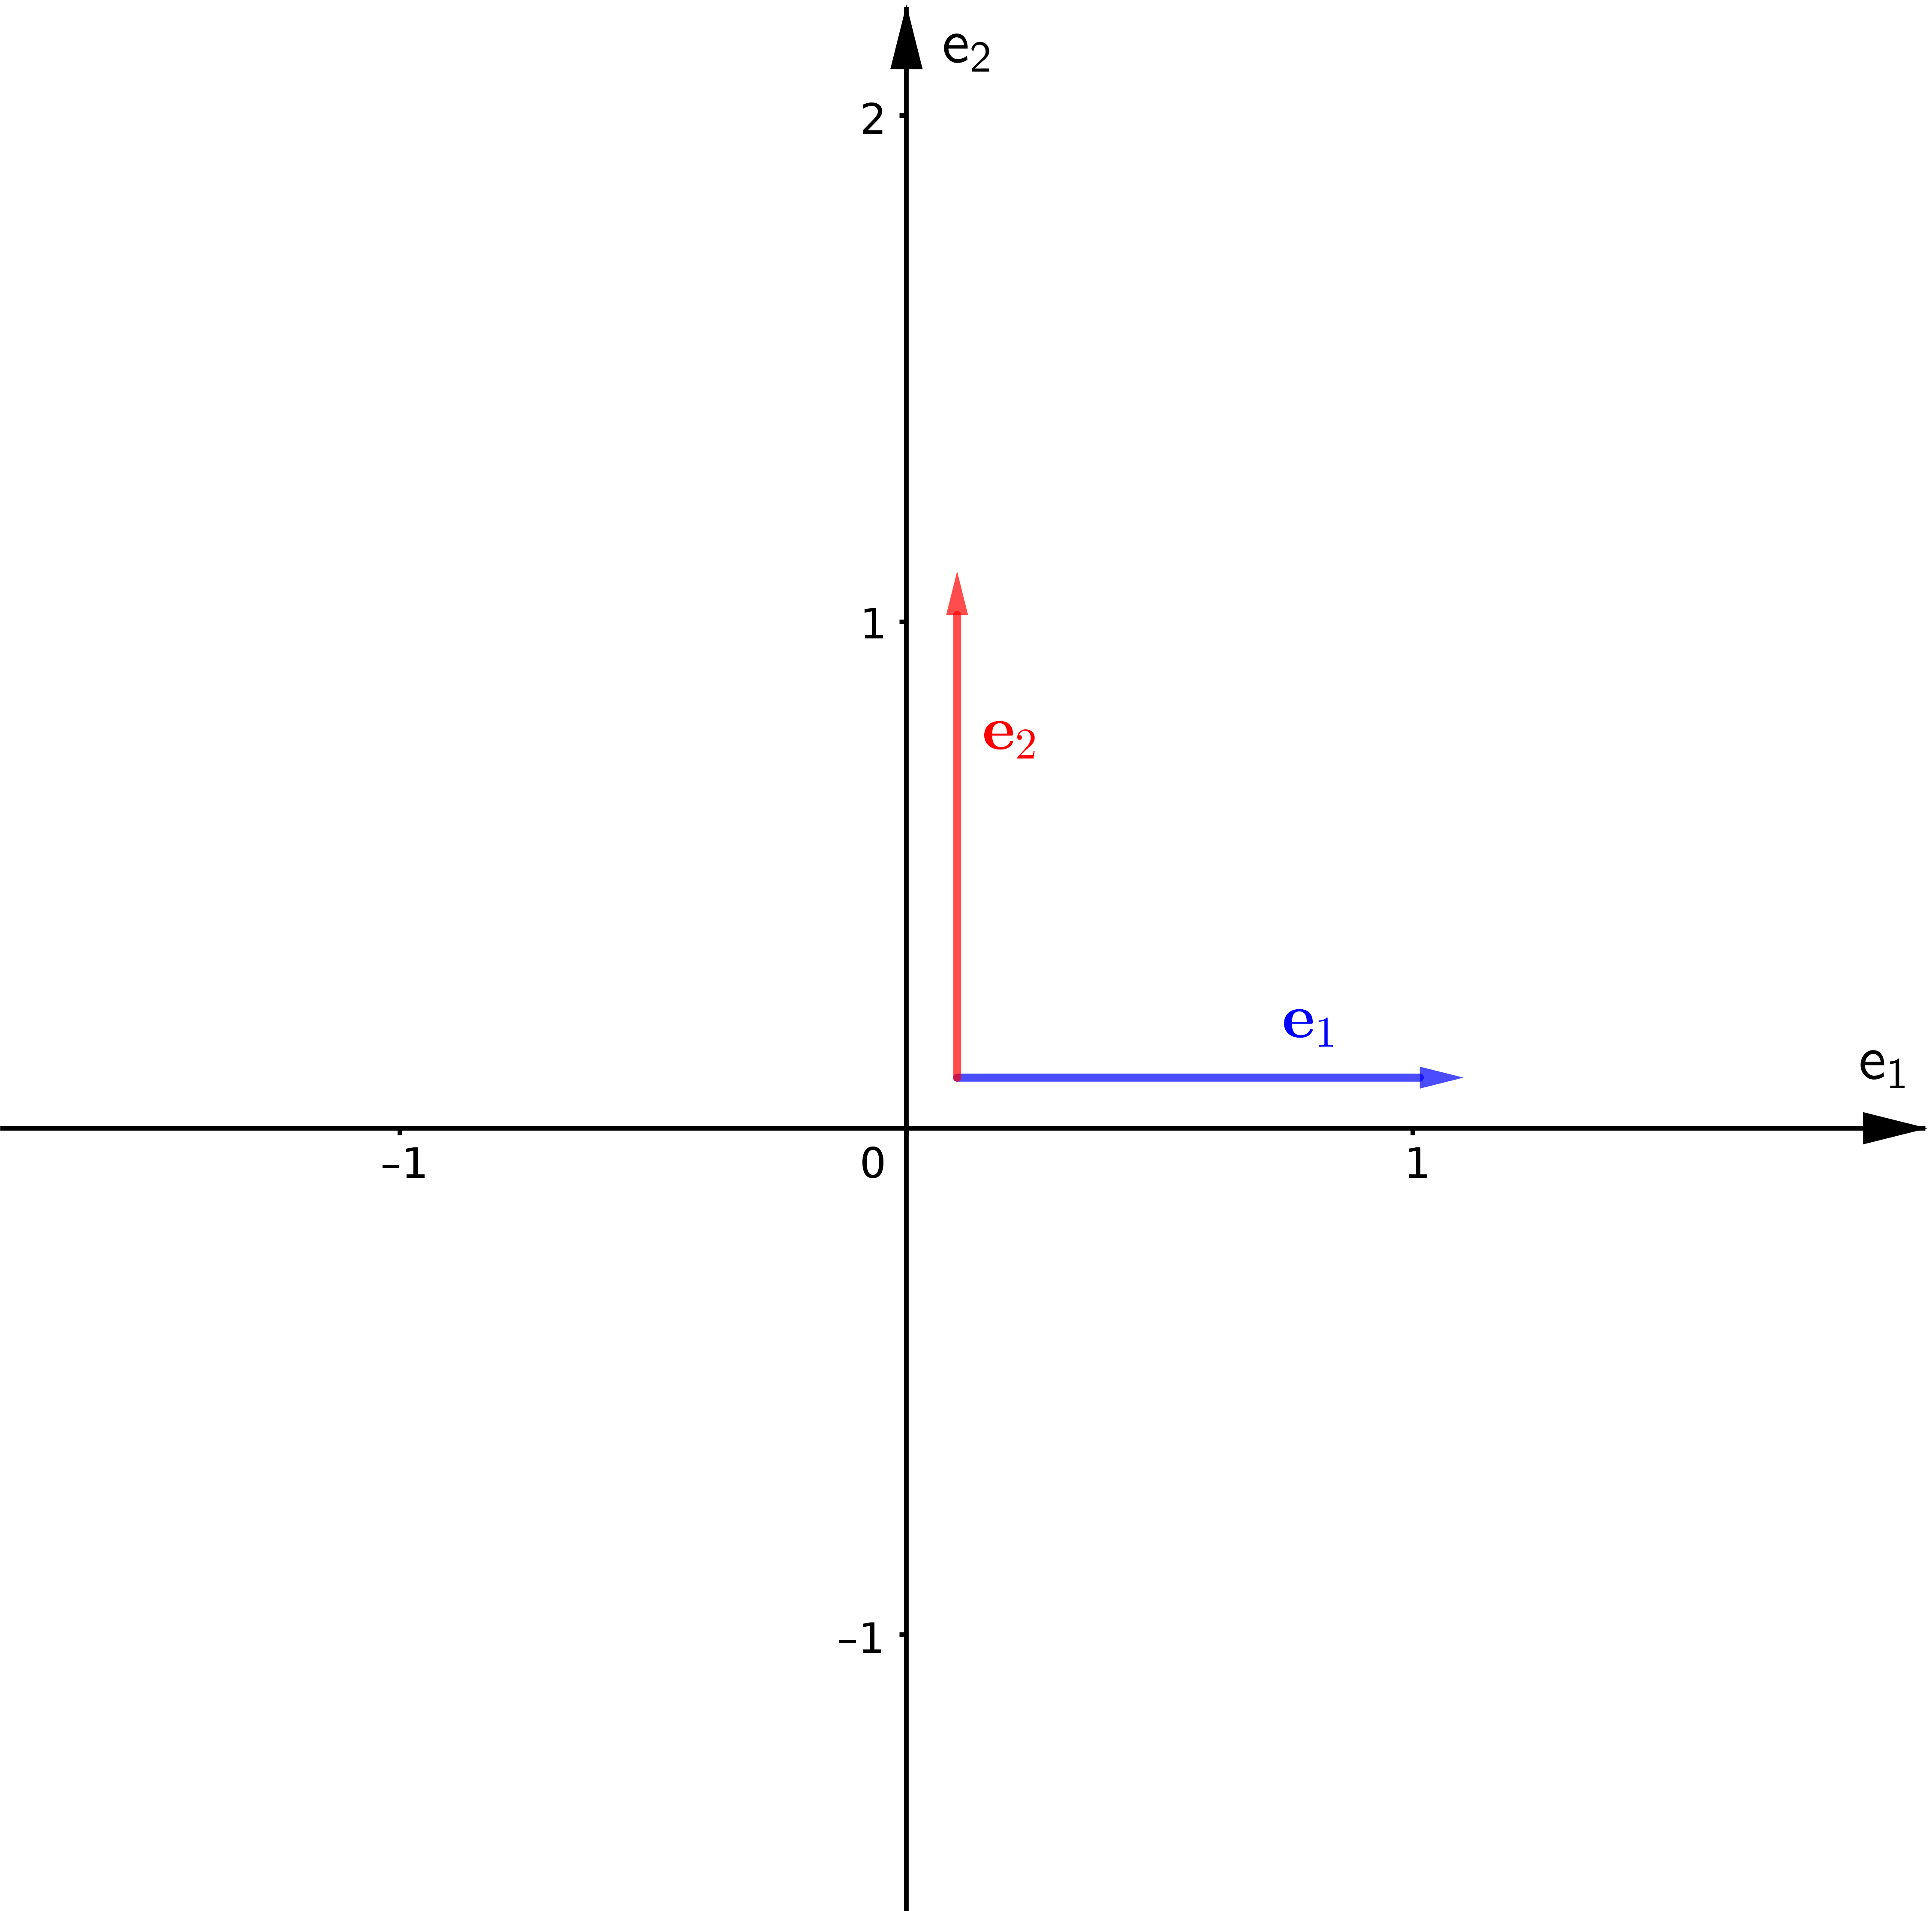
\includegraphics[width=0.7\textwidth,height=\textheight]{figures/vetores-base.png}

  }

  \caption{\label{fig-e1-e2}Vetores da base canônica e eixos}

  \end{figure}

  \begin{tcolorbox}[standard jigsaw,toprule=.15mm, bottomrule=.15mm, opacityback=0, toptitle=1mm, bottomtitle=1mm, colbacktitle=quarto-callout-warning-color!10!white, left=2mm, titlerule=0mm, title=\textcolor{quarto-callout-warning-color}{\faExclamationTriangle}\hspace{0.5em}{Notação: vetores como combinações lineares dos vetores da base}, arc=.35mm, rightrule=.15mm, colback=white, coltitle=black, colframe=quarto-callout-warning-color-frame, opacitybacktitle=0.6, leftrule=.75mm]
  Como na maioria dos livros sobre álgebra geométrica, em vez de
  escrevermos \[
  \mathbf{v} = (x, y)
  \] vamos escrever \[
  \mathbf{v} = x\mathbf{e}_{1} + y\mathbf{e}_{2}
  \]

  Se uma das coordenadas for zero, podemos omitir o vetor da base
  correspondente. Por exemplo, vamos escrever o vetor \[
  \mathbf{u} = (0, 3)
  \] como \[
  \mathbf{u} = 3\mathbf{e}_{2}
  \]
  \end{tcolorbox}
\item
  \protect\hypertarget{topicos-vetores}{}{} Para acompanhar o restante
  deste capítulo, você deve revisar os seguintes tópicos sobre vetores,
  especialmente em $\mathbb{R}^2$ e em $\mathbb{R}^3$:

  \begin{itemize}
  \tightlist
  \item
    Adição de vetores,
  \item
    Multiplicação de vetor por escalar (nossos escalares vão ser números
    reais),
  \item
    Vetor nulo,
  \item
    Vetor inverso (para a adição),
  \item
    Dependência e independência linear,
  \item
    Módulo (norma) de um vetor,
  \item
    Produto vetorial,
  \item
    Subespaços vetoriais.
  \end{itemize}
\end{itemize}

\hypertarget{retas-em-mathbbr2}{%
\section{\texorpdfstring{Retas em
$\mathbb{R}^2$}{Retas em }}\label{retas-em-mathbbr2}}

\begin{itemize}
\item
  Por enquanto, só temos vetores.
\item
  Cada vetor (diferente de $\mathbf{0}$, o vetor nulo) indica uma
  direção.
\item
  Mas apenas uma direção não basta para definir uma reta. Por exemplo,
  todas as retas da Figura~\ref{fig-retas} têm a mesma direção: a
  direção dada pelo vetor
  $\mathbf{v} = \mathbf{e}_{1} + 2\mathbf{e}_{2}$.

  \begin{figure}[t]

  {\centering 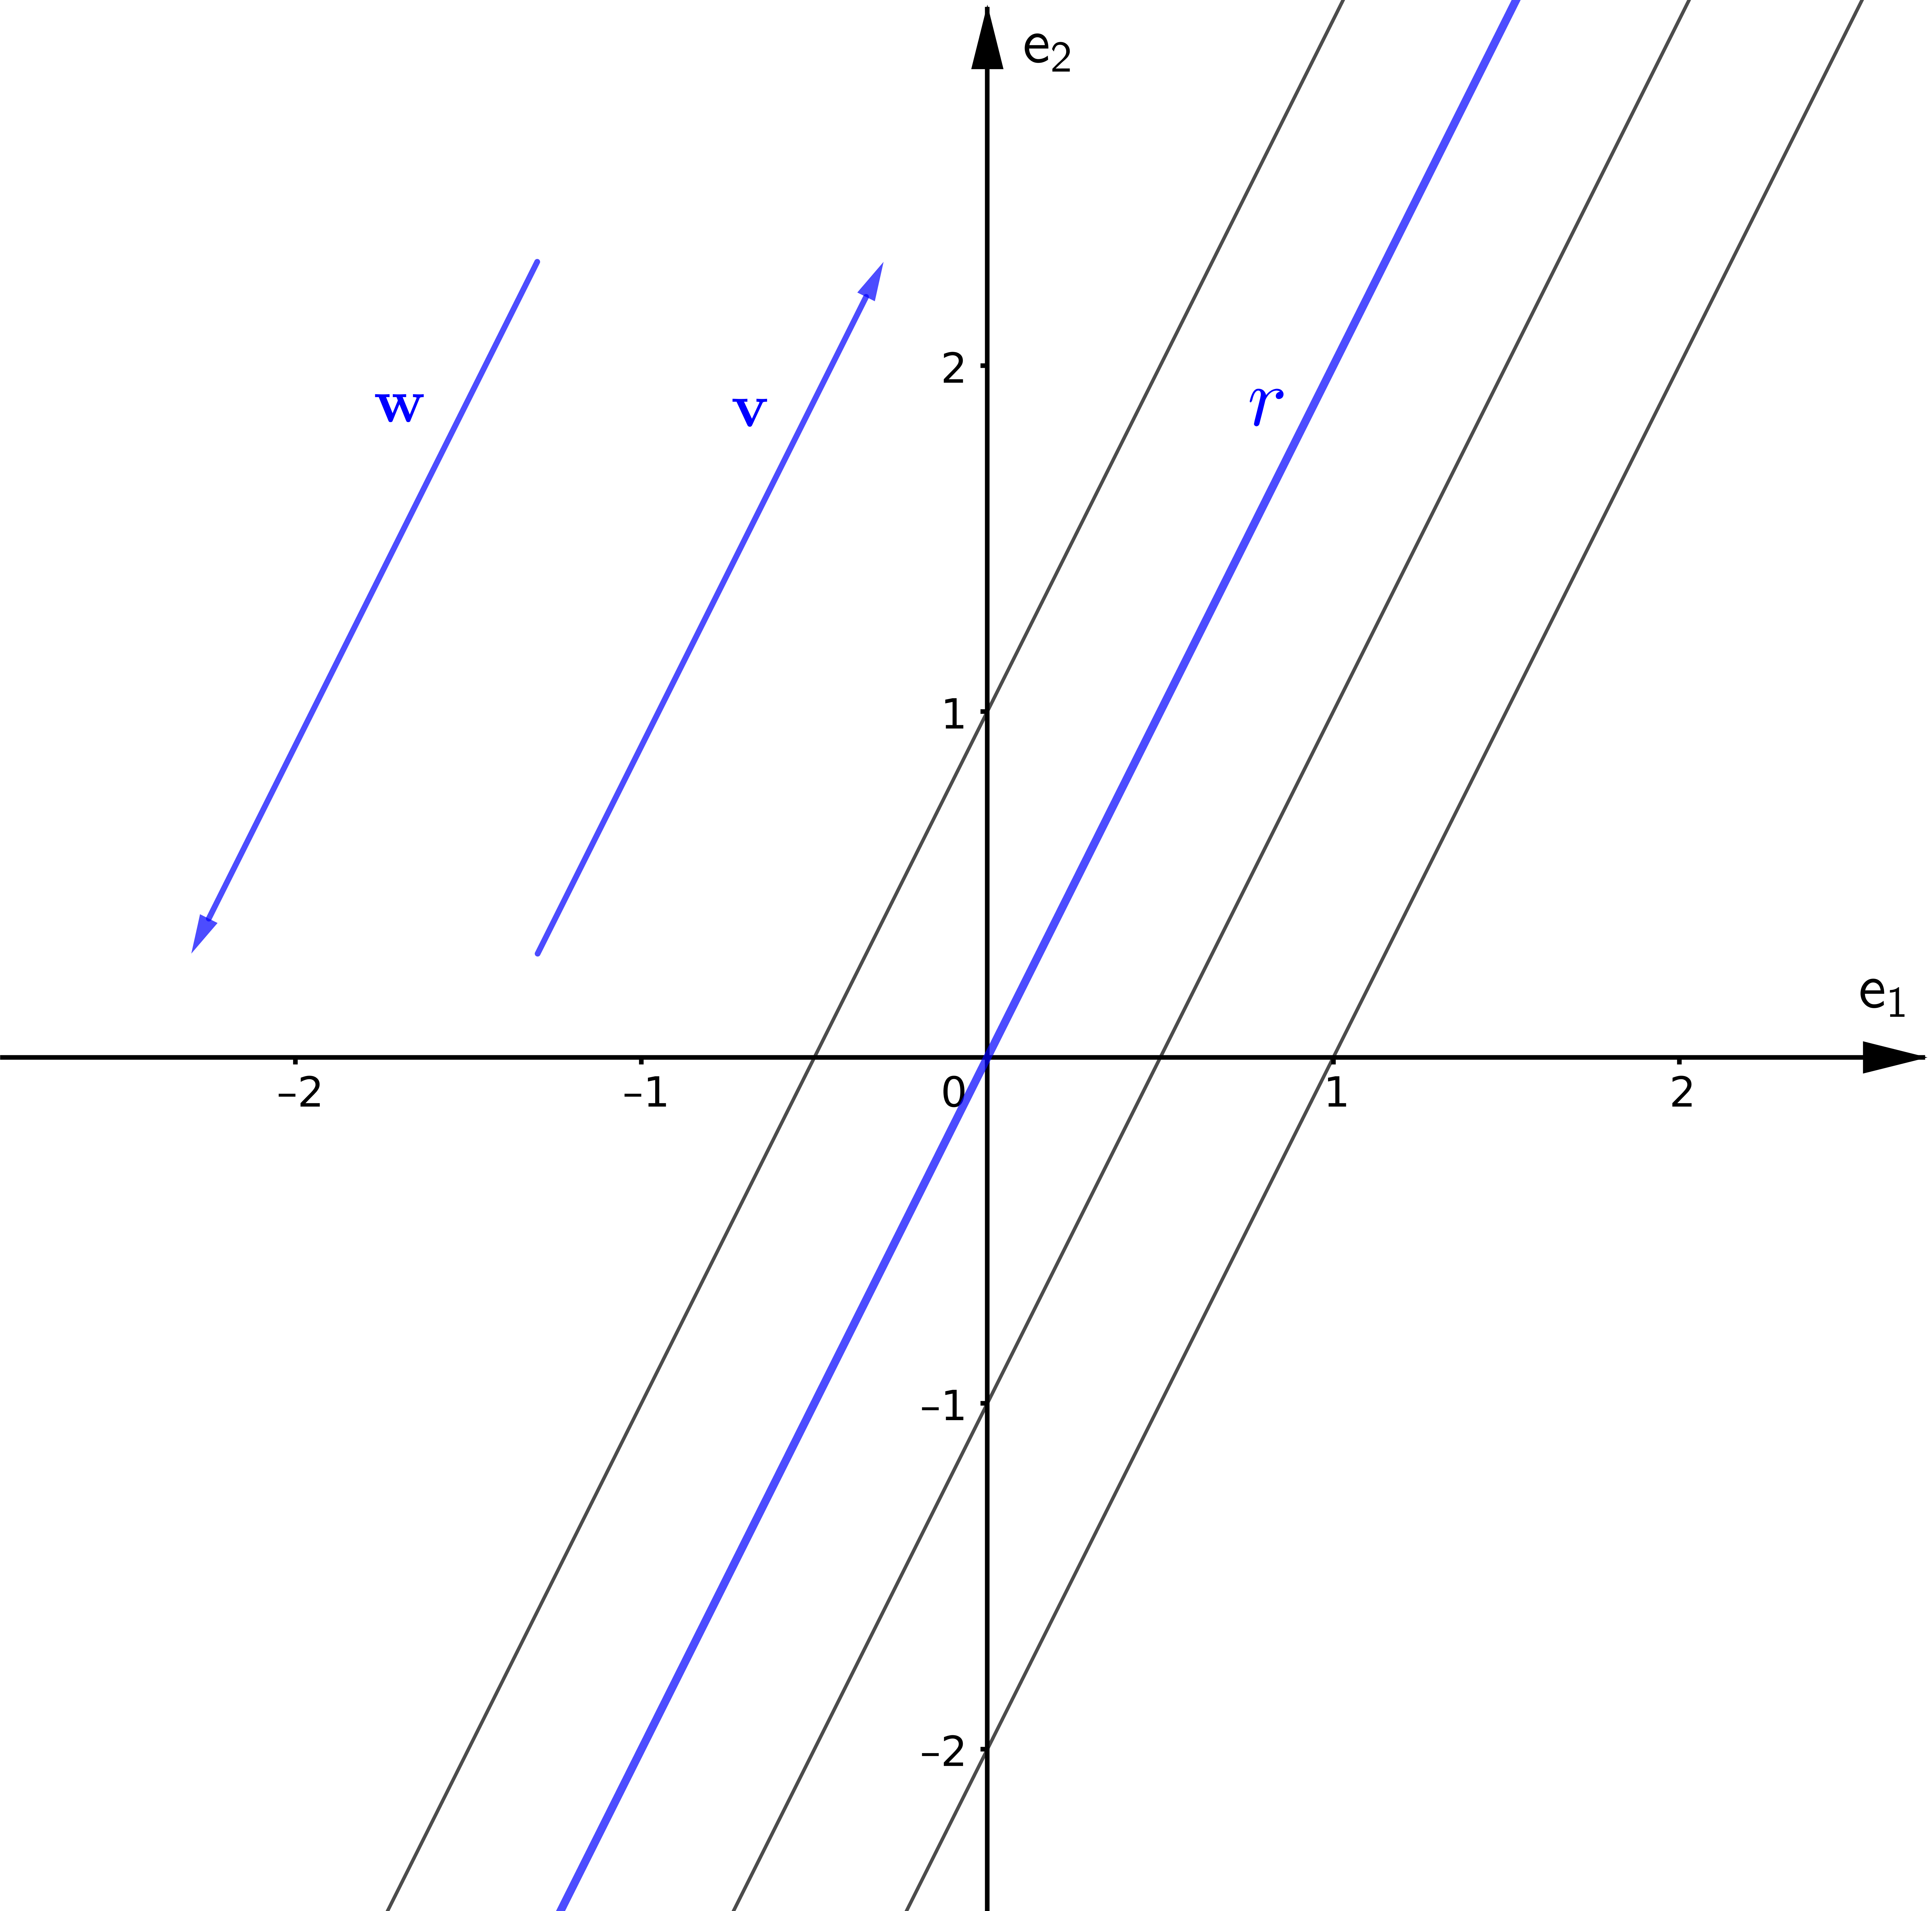
\includegraphics[width=0.8\textwidth,height=\textheight]{figures/reta-homogenea.png}

  }

  \caption{\label{fig-retas}Retas e vetores}

  \end{figure}
\item
  Vamos combinar que {\hl{todas as nossas retas de interesse passam pela
  origem}} --- ou seja, pelo ponto $O=(0,0)$.
\item
  Fazendo isto, cada vetor determina uma única reta.
\item
  Chamamos as retas que passam pela origem de {\hl{retas homogêneas}}.
  Na Figura~\ref{fig-retas}, só há uma reta homogênea (a reta $r$).
\item
  Mas, além de uma direção, um vetor também um {\hl{sentido}}.
\item
  Na Figura~\ref{fig-retas}, o vetor
  $\mathbf{w} = -\mathbf{e}_{1} - 2\mathbf{e}_{2}$ tem a mesma direção
  da reta $r$, mas seu sentido é oposto ao sentido do vetor
  $\mathbf{v}$.
\item
  Então, {\hl{qual dos dois vetores $\mathbf{v}$ e $\mathbf{w}$
  representa a reta $r$?}}
\item
  Vamos decidir esta questão do seguinte modo: {\hl{nossas retas também
  vão ter um sentido}}. Ou seja, vamos trabalhar com {\hl{retas
  orientadas}}.
\item
  Na Figura~\ref{fig-retas}, então, os vetores $\mathbf{v}$ e
  $\mathbf{w}$ representam duas retas $r$ e $r'$, ambas com a mesma
  direção, mas com sentidos opostos.
\item
  Mas, além de direção e sentido, um vetor também tem um
  {\hl{comprimento}} (ou {\hl{magnitude}}, ou {\hl{módulo}}, ou
  {\hl{norma}}).
\item
  Na Figura~\ref{fig-vetores}, os $3$ vetores
  $\mathbf{v}_1, \mathbf{v}_2$ e $\mathbf{v}_3$ têm a mesma direção e
  sentido que a reta $r$.

  \begin{figure}[t]

  {\centering 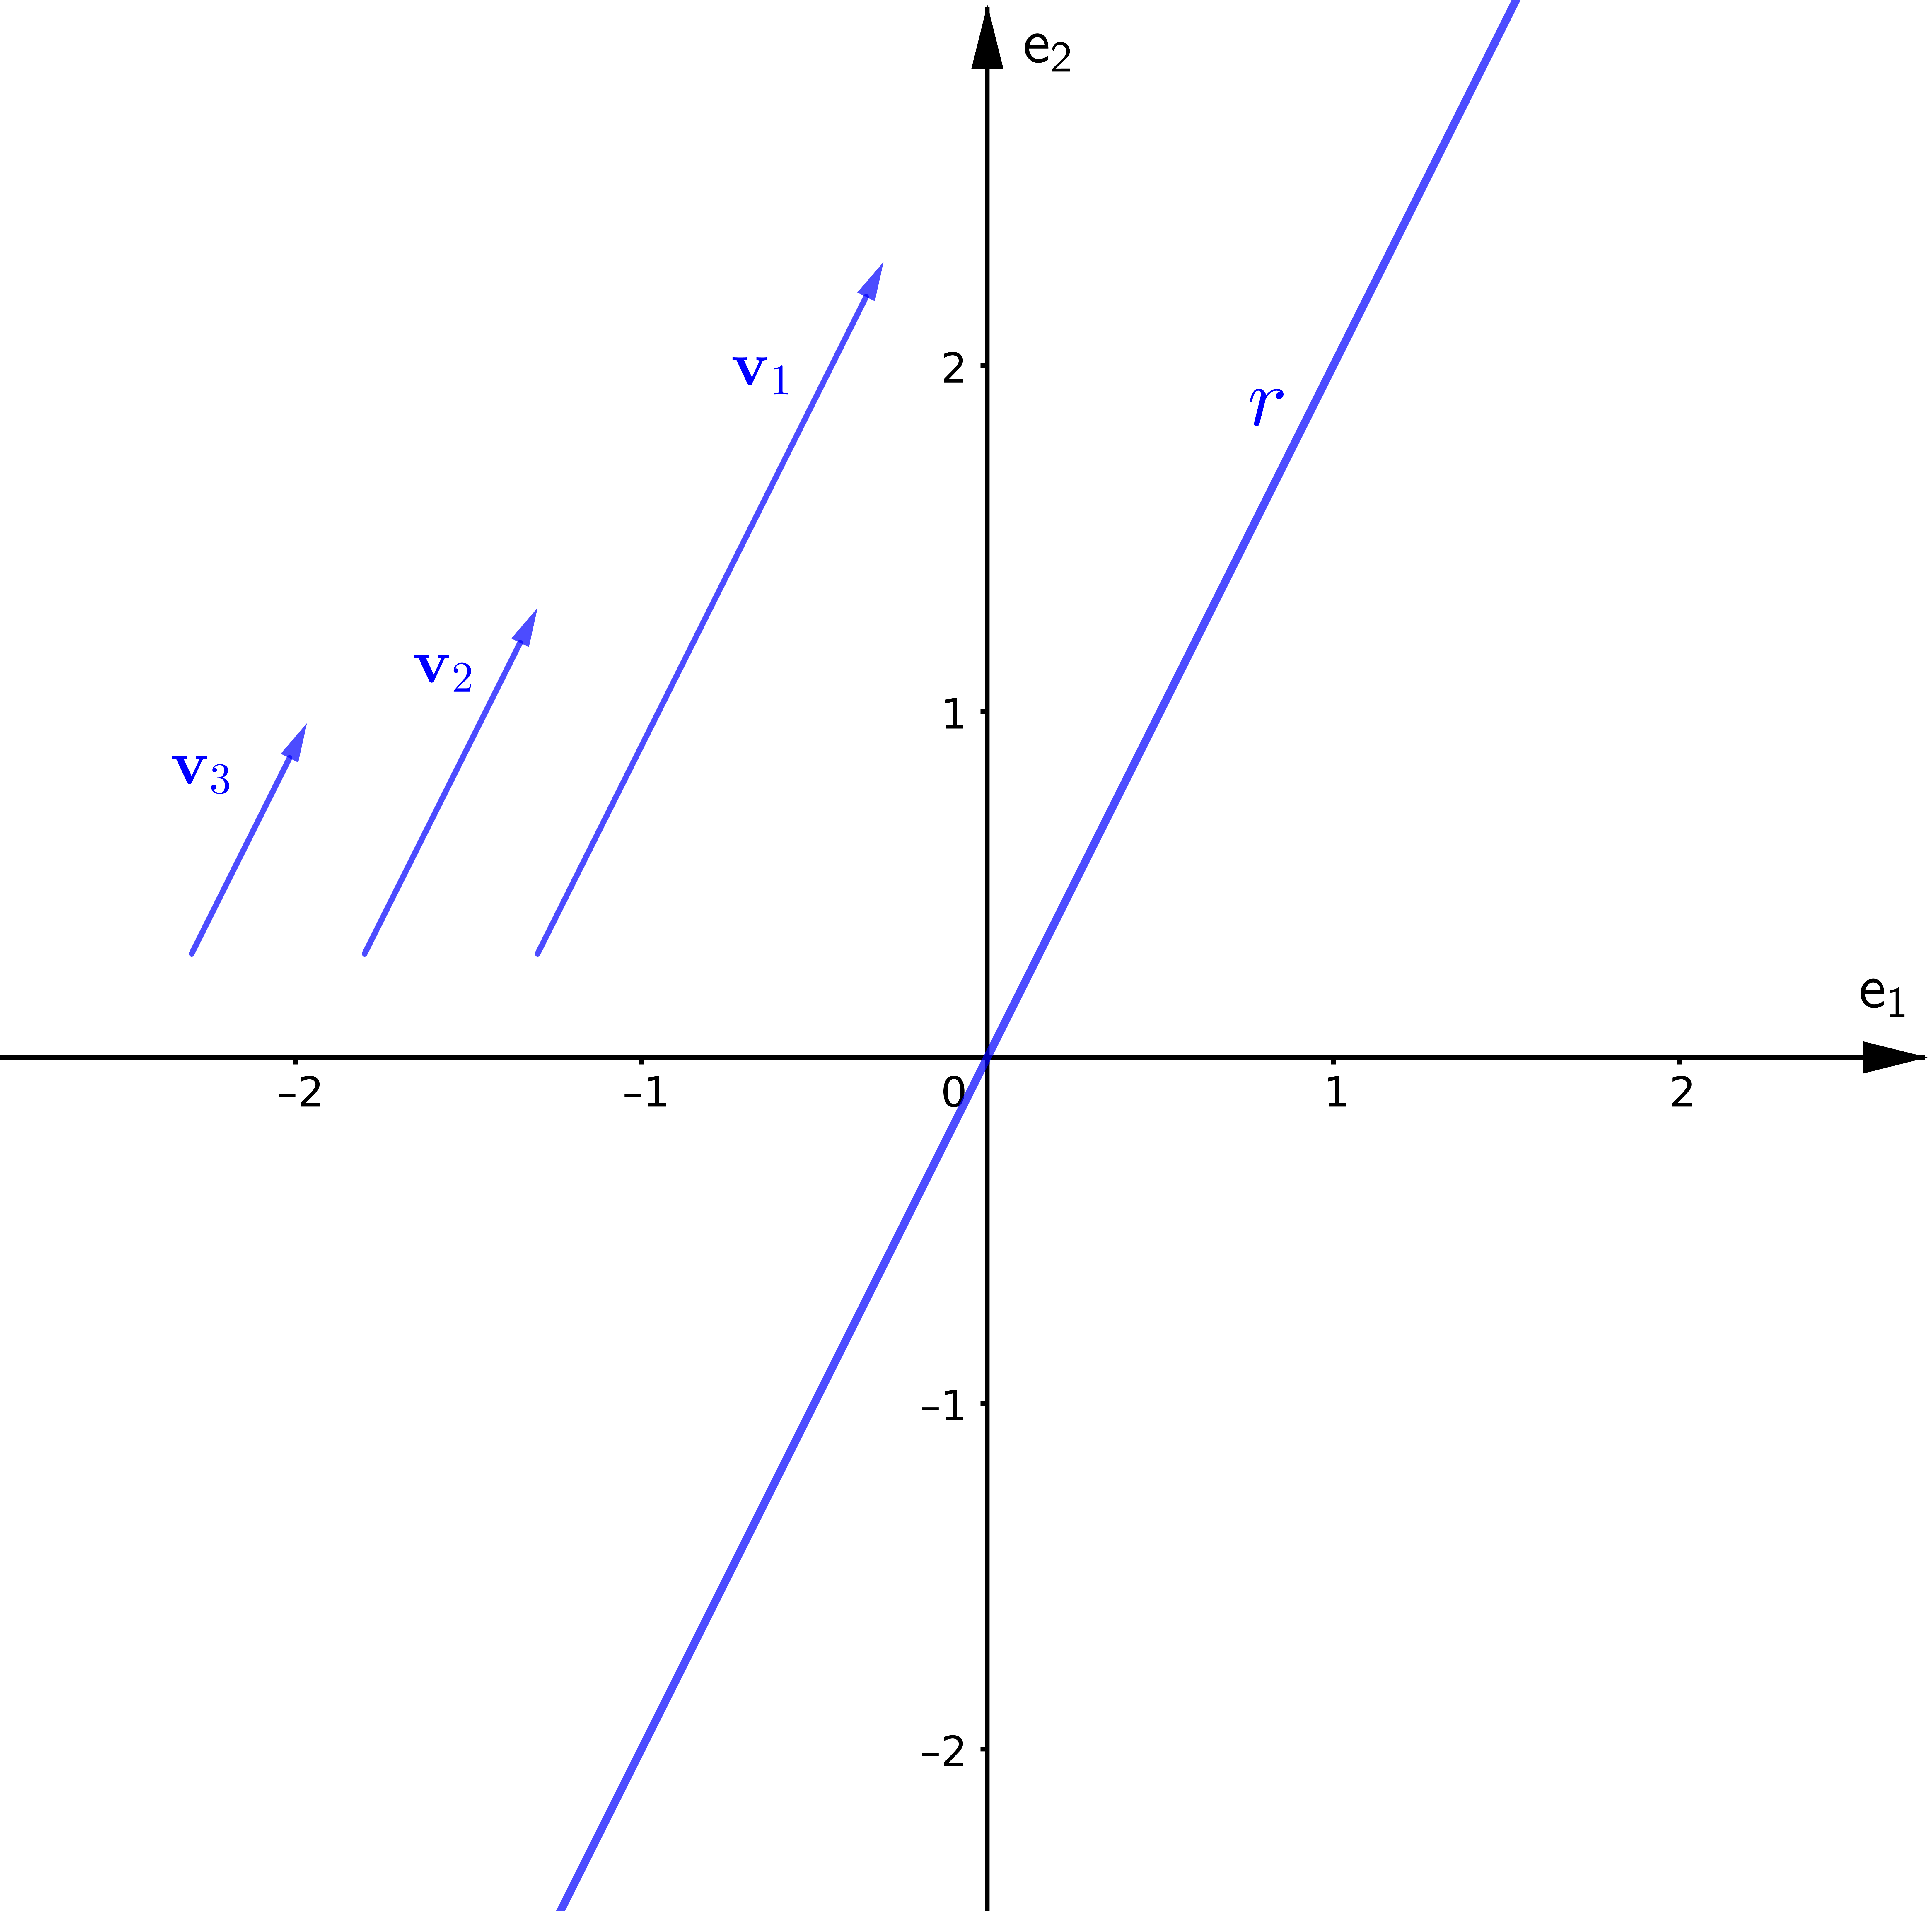
\includegraphics[width=0.8\textwidth,height=\textheight]{figures/reta-vetores.png}

  }

  \caption{\label{fig-vetores}Vetores de magnitudes diferentes}

  \end{figure}
\item
  De novo, vamos combinar que {\hl{cada um destes vetores define uma
  reta diferente}}, todas as retas com a mesma direção e sentido, mas
  {\hl{cada reta com uma magnitude (ou peso) diferente}}.
\item
  Você pode imaginar o peso de uma reta como a {\hl{velocidade}} com que
  um ponto percorre a reta, ou como a {\hl{velocidade}} com que a reta
  avança na direção e no sentido especificados pelo vetor.

  \begin{tcolorbox}[standard jigsaw,toprule=.15mm, bottomrule=.15mm, opacityback=0, toptitle=1mm, bottomtitle=1mm, colbacktitle=quarto-callout-note-color!10!white, left=2mm, titlerule=0mm, title=\textcolor{quarto-callout-note-color}{\faInfo}\hspace{0.5em}{Resumindo: vetores \(=\) retas homogêneas orientadas e com peso}, arc=.35mm, rightrule=.15mm, colback=white, coltitle=black, colframe=quarto-callout-note-color-frame, opacitybacktitle=0.6, leftrule=.75mm]
  Um vetor \[
  \mathbf{v} = a\mathbf{e}_{1} + b\mathbf{e}_{2}
  \] (com $a, b \in \mathbb{R}$, e com pelo menos um dentre $a$ e $b$
  diferente de zero) {\hl{representa uma reta homogênea orientada, com a
  direção e o sentido de $\mathbf{v}$, e com peso igual à norma de
  $\mathbf{v}$:}} \[
  ||\mathbf{v}|| = \sqrt{a^2 + b^2}
  \]
  \end{tcolorbox}
\end{itemize}

\hypertarget{vetores-e-retas-em-mathbbr3}{%
\section{\texorpdfstring{Vetores e retas em
$\mathbb{R}^3$}{Vetores e retas em }}\label{vetores-e-retas-em-mathbbr3}}

\begin{itemize}
\item
  Agora, vamos trabalhar em $\mathbb{R}^3$.
\item
  Tudo que falamos acima sobre vetores e retas em $\mathbb{R}^2$ se
  aplica a vetores e retas em $\mathbb{R}^3$, com as seguintes
  alterações:

  \begin{itemize}
  \item
    A base canônica agora é
    $\{ \mathbf{e}_{1}, \mathbf{e}_{2}, \mathbf{e}_{3} \}$, onde os
    vetores correspondem aos eixos $x$, $y$ e $z$, respectivamente.
  \item
    Logo, um vetor em $\mathbb{R}^3$ é escrito como
    $\mathbf{v} = x\mathbf{e}_{1} + y\mathbf{e}_{2} + z\mathbf{e}_{3}$,
    com $x, y, z \in \mathbb{R}$.
  \item
    Cada vetor
    $\mathbf{v} = a\mathbf{e}_{1} + b\mathbf{e}_{2} + c\mathbf{e}_{3}$
    (com $a, b, c \in \mathbb{R}$, e com pelo menos um dentre $a$, $b$ e
    $c$ diferente de zero) representa uma reta homogênea orientada, com
    a direção e o sentido de $\mathbf{v}$, e com peso igual à norma de
    $\mathbf{v}$: \[
    ||\mathbf{v}|| = \sqrt{a^2 + b^2 + c^2}
    \]
  \end{itemize}
\item
  A Figura~\ref{fig-reta-r3} mostra um exemplo.

  \begin{figure}[t]

  {\centering 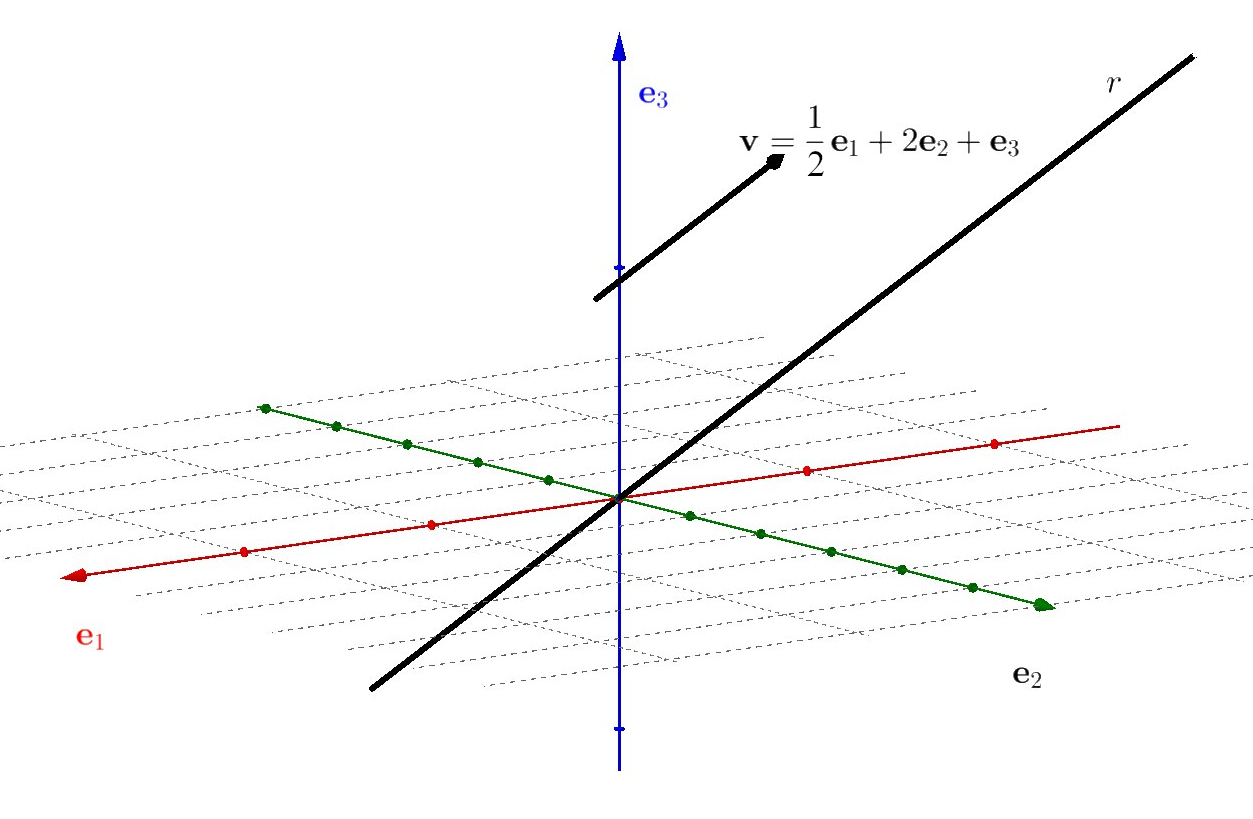
\includegraphics[width=1\textwidth,height=\textheight]{figures/reta-r3.png}

  }

  \caption{\label{fig-reta-r3}Vetor e reta em $\mathbb{R}^3$}

  \end{figure}
\end{itemize}

\hypertarget{bivetores-e-planos-em-mathbbr3}{%
\section{\texorpdfstring{Bivetores e planos em
$\mathbb{R}^3$}{Bivetores e planos em }}\label{bivetores-e-planos-em-mathbbr3}}

\begin{itemize}
\item
  Agora, ainda em $\mathbb{R}^3$, considere planos {\hl{homogêneos}}
  (que contêm a origem).
\item
  Um plano homogêneo neste espaço tridimensional é definido por dois
  vetores linearmente independentes (isto é, com direções diferentes).
\item
  Por exemplo, o plano da Figura~\ref{fig-plano} é definido pelos
  vetores
  $\mathbf{v} = \mathbf{e}_{1} + 2\mathbf{e}_{2} + \mathbf{e}_{3}$ e
  $\mathbf{w} = 3\mathbf{e}_{1} - \mathbf{e}_{2}$.

  \begin{figure}[t]

  {\centering 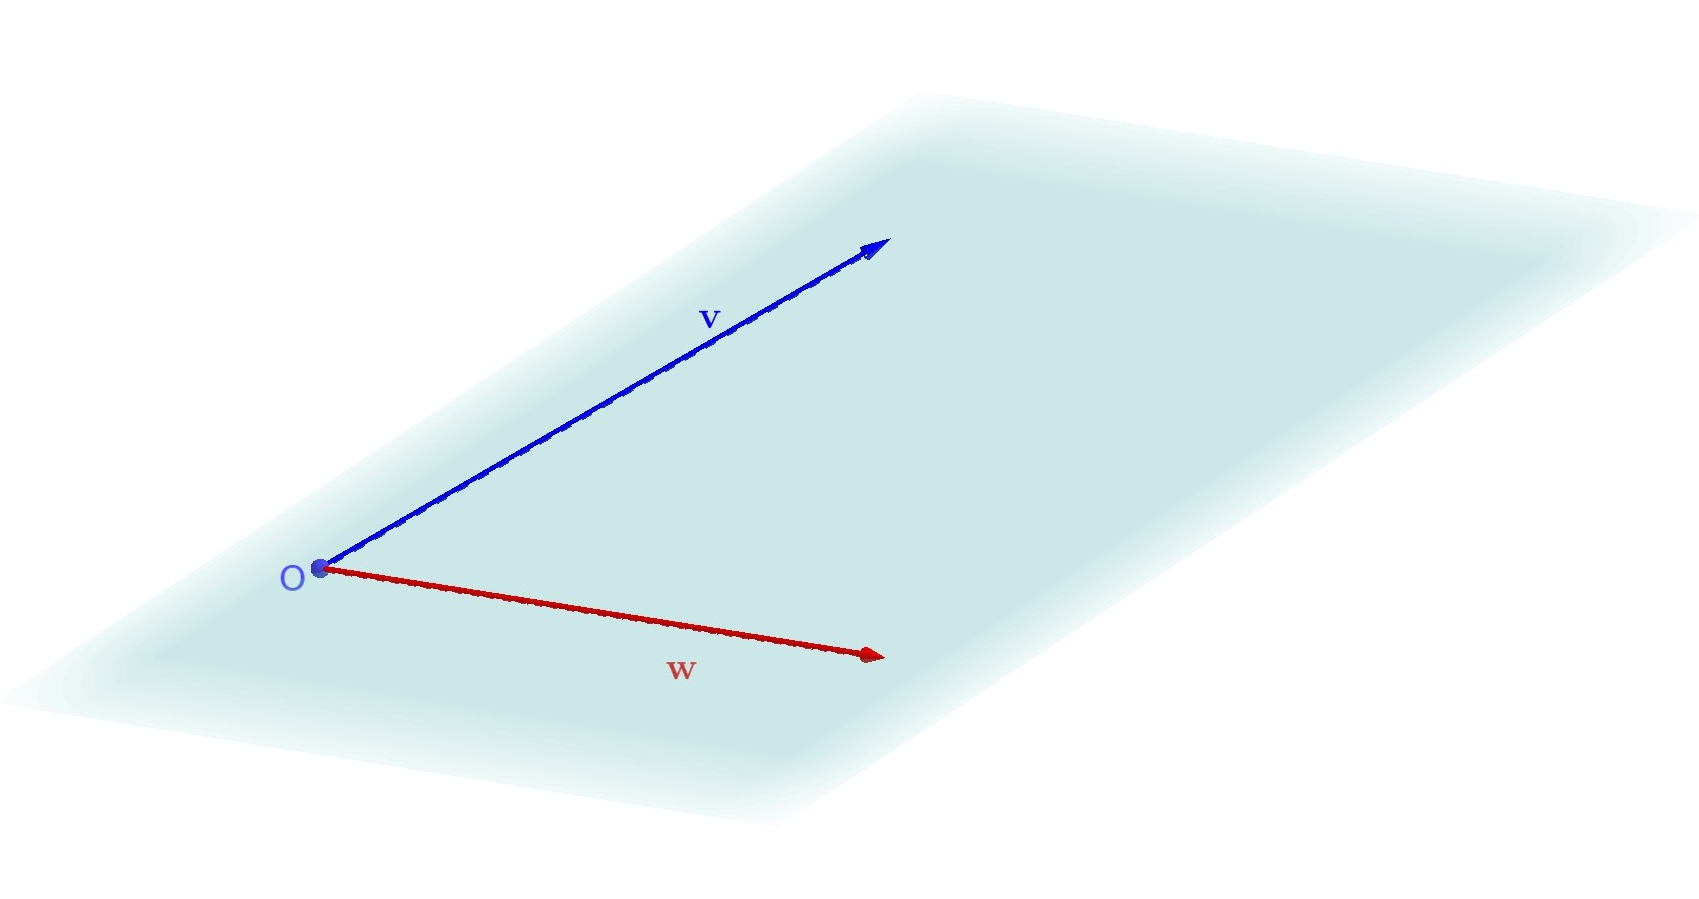
\includegraphics[width=1\textwidth,height=\textheight]{figures/plano.jpg}

  }

  \caption{\label{fig-plano}Plano homogêneo em $\mathbb{R}^3$}

  \end{figure}
\item
  De novo, como fizemos antes com as retas, {\hl{vamos querer levar em
  conta os sentidos e as normas}} destes dois vetores na maneira como
  eles definem um plano.
\item
  Quanto aos sentidos: vamos dizer que o plano gerado por estes dois
  vetores pode ter {\hl{duas orientações}}, dependendo da {\hl{ordem em
  que tomarmos os vetores}}.
\item
  Detalhando: o plano gerado por $\mathbf{v}$ e $\mathbf{w}$ (nesta
  ordem) vai ter uma orientação, e o plano gerado por $\mathbf{w}$ e
  $\mathbf{v}$ (nesta ordem) vai ter a orientação oposta.
\item
  Se você revisou os \protect\hyperlink{topicos-vetores}{tópicos
  recomendados sobre vetores}, você deve estar lembrando que o
  {\hl{produto vetorial}} tem um comportamento parecido:
\item
  Quando $\mathbf{v}$ e $\mathbf{w}$ são linearmente independentes, o
  resultado do produto vetorial $\mathbf{v} \times \mathbf{w}$ é um
  vetor {\hl{perpendicular}} ao plano definido por $\mathbf{v}$ e
  $\mathbf{w}$.
\item
  O resultado do produto vetorial $\mathbf{v} \times \mathbf{w}$ é um
  vetor que tem o {\hl{sentido oposto}} ao resultado do produto vetorial
  $\mathbf{w} \times \mathbf{v}$. O sentido de cada resultado é dado
  pela regra da mão direita.
\item
  Além disso, a {\hl{norma}} do produto vetorial
  $\mathbf{v} \times \mathbf{w}$ --- que é igual à norma do produto
  vetorial $\mathbf{w} \times \mathbf{v}$ --- tem o mesmo valor do que a
  {\hl{área do paralelogramo}} definido por $\mathbf{v}$ e $\mathbf{w}$.
  Veja a Figura~\ref{fig-prod-vet}.

  \begin{figure}[t]

  {\centering 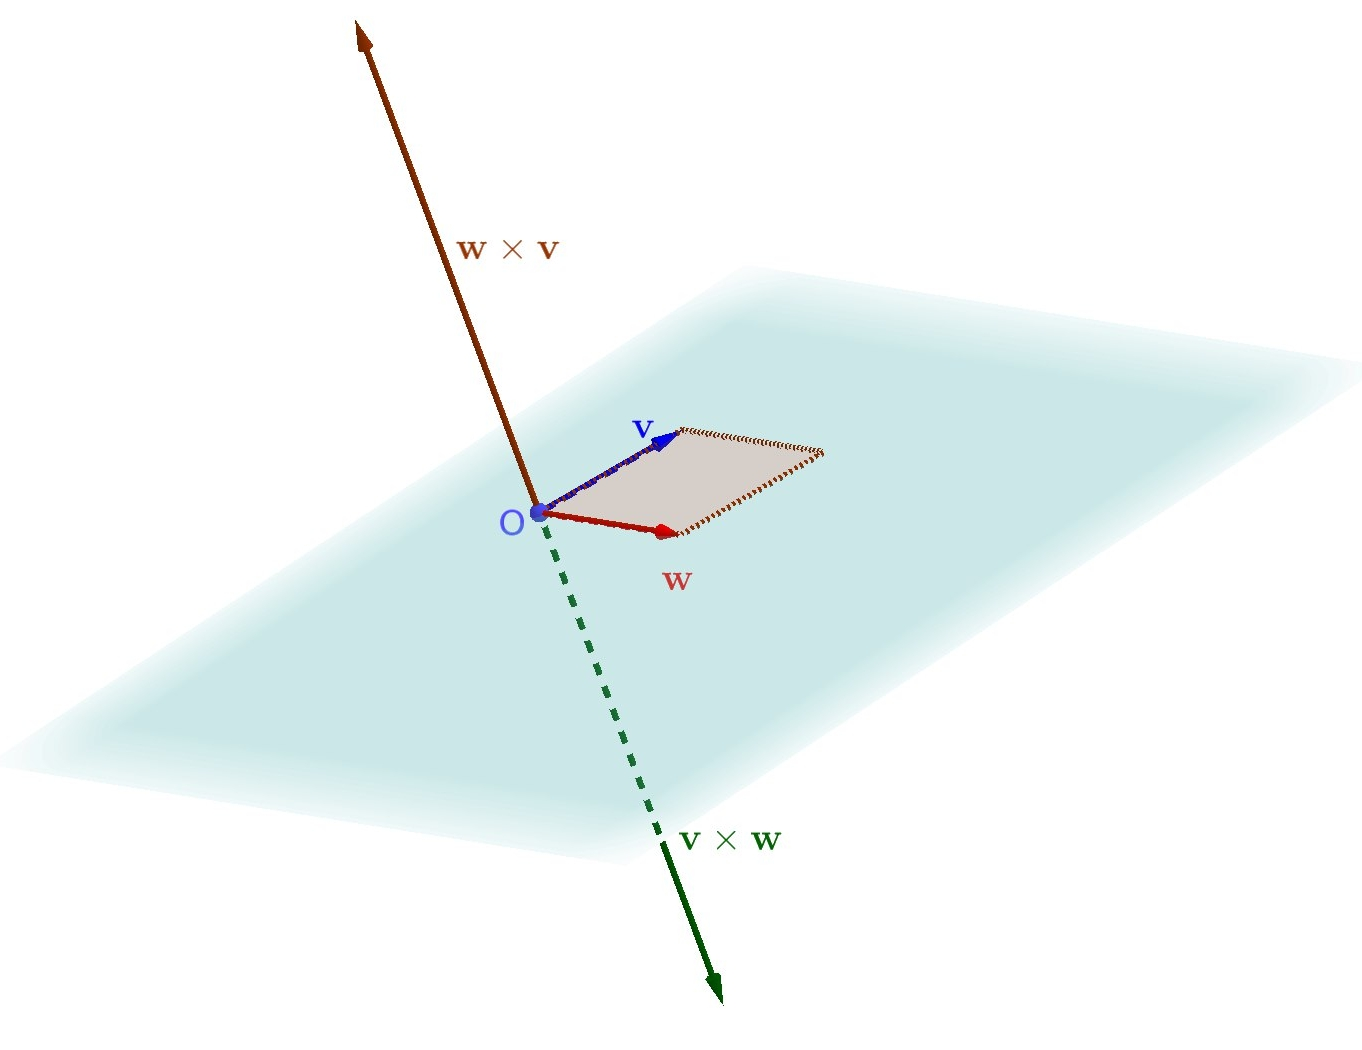
\includegraphics[width=1\textwidth,height=\textheight]{figures/prod-vet.jpg}

  }

  \caption{\label{fig-prod-vet}Produtos vetoriais}

  \end{figure}
\item
  Com isto, temos tudo de que precisamos para definir planos homogêneos
  que, além de direção, têm {\hl{peso}} (magnitude) e {\hl{orientação}}
  (sentido):
\item
  O {\hl{peso}} do plano definido por $\mathbf{v}$ e $\mathbf{w}$ tem o
  mesmo valor absoluto da {\hl{área do paralelogramo}}, com o sinal
  positivo ou negativo, dependendo da regra da mão direita. Na
  Figura~\ref{fig-prod-vet}, o peso do plano definido por $\mathbf{v}$ e
  $\mathbf{w}$ (nesta ordem) é {\hl{negativo}}, e o peso do plano
  definido por $\mathbf{w}$ e $\mathbf{v}$ (nesta ordem) é
  {\hl{positivo}}.
\item
  A {\hl{orientação}} do plano definido por $\mathbf{v}$ e $\mathbf{w}$
  (nesta ordem) é oposta à orientação do plano definido por $\mathbf{w}$
  e $\mathbf{v}$ (nesta ordem).
\item
  {\hl{Vamos chamar de bivetor}} este plano homogêneo, orientado e com
  peso.
\item
  A Figura~\ref{fig-bivetor-wv} mostra o bivetor definido por
  $\mathbf{w}$ e $\mathbf{v}$ (nesta ordem). A orientação é dada por uma
  seta circular.

  \begin{figure}[t]

  {\centering 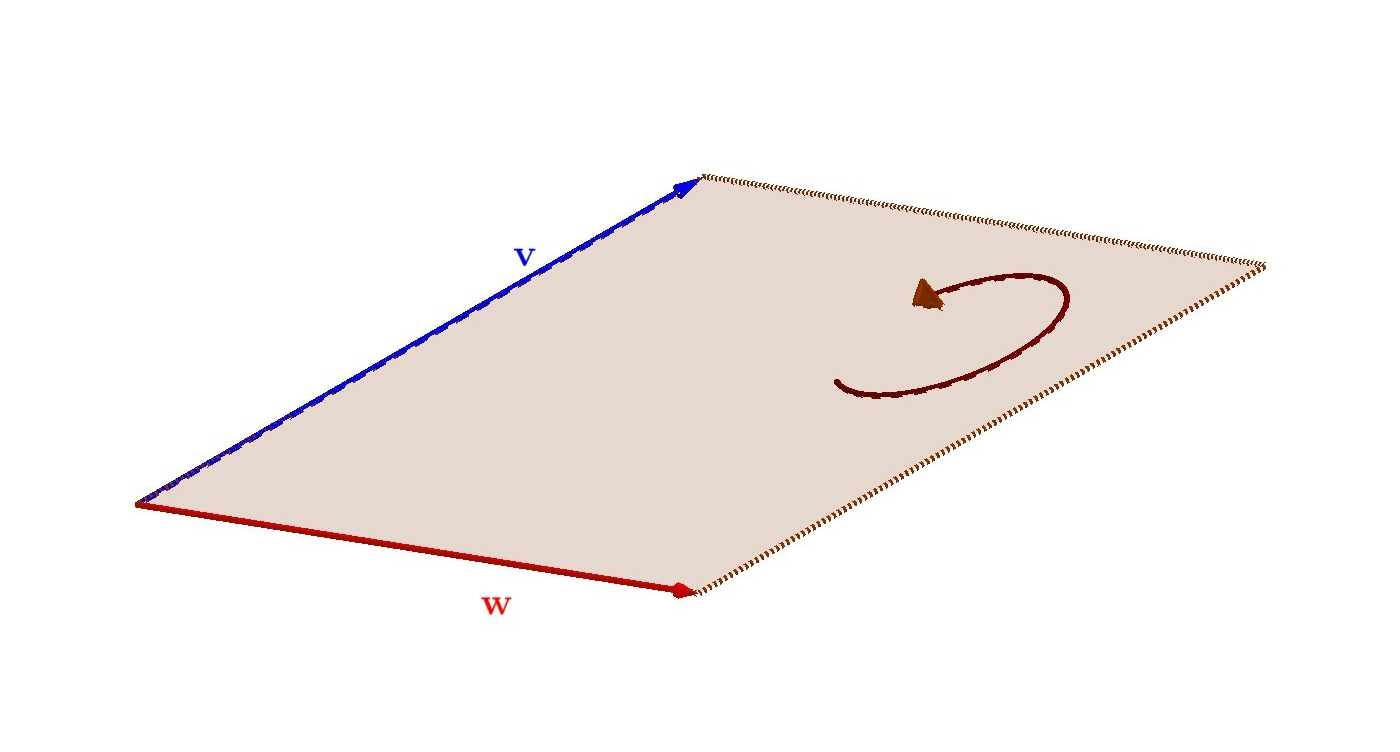
\includegraphics[width=1\textwidth,height=\textheight]{figures/bivetor-wv.jpg}

  }

  \caption{\label{fig-bivetor-wv}Bivetor definido por $\mathbf{w}$ e
  $\mathbf{v}$ (nesta ordem)}

  \end{figure}
\item
  A Figura~\ref{fig-bivetor-vw} mostra o bivetor definido por
  $\mathbf{v}$ e $\mathbf{w}$ (nesta ordem). A orientação é oposta à do
  bivetor na Figura~\ref{fig-bivetor-wv}.

  \begin{figure}[t]

  {\centering 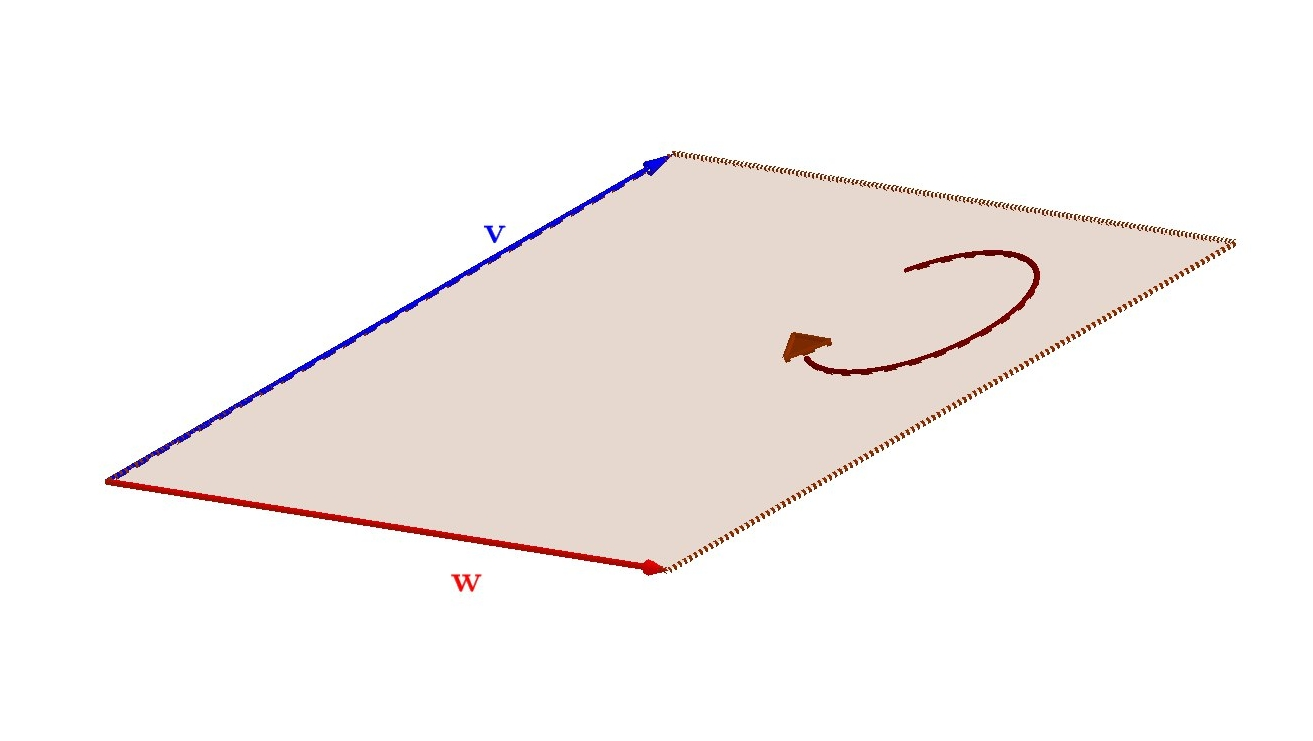
\includegraphics[width=1\textwidth,height=\textheight]{figures/bivetor-vw.jpg}

  }

  \caption{\label{fig-bivetor-vw}Bivetor definido por $\mathbf{v}$ e
  $\mathbf{w}$ (nesta ordem)}

  \end{figure}
\item
  Nas figuras, representamos um bivetor como uma {\hl{área orientada}}
  em um plano.
\item
  Mas {\hl{a forma desta área não é importante}}. As figuras mostram
  paralelogramos, mas os mesmos bivetores poderiam ser mostrados como
  círculos, triângulos etc. com a mesma área.
\item
  As figuras parecem diferenciar planos (que são infinitos) e bivetores
  (que têm, associados a eles, áreas finitas). Mais adiante, vamos ver
  que, em algumas aplicações, {\hl{podemos interpretar um bivetor como
  representando o plano no qual ele está contido}}; em outras
  aplicações, {\hl{podemos interpretar um bivetor como uma porção finita
  do plano}}.
\end{itemize}

\hypertarget{o-produto-externo-de-vetores-cria-bivetores}{%
\section{O produto externo de vetores cria
bivetores}\label{o-produto-externo-de-vetores-cria-bivetores}}

???

Notação

Antissimetria

Vetores paralelos

Distributividade

Exemplos numéricos

\hypertarget{bivetores-em-mathbbr2}{%
\section{\texorpdfstring{Bivetores em
$\mathbb{R}^2$?}{Bivetores em ?}}\label{bivetores-em-mathbbr2}}

\hypertarget{trivetores-em-mathbbr3}{%
\section{\texorpdfstring{Trivetores em
$\mathbb{R}^3$}{Trivetores em }}\label{trivetores-em-mathbbr3}}

\hypertarget{k-vetores-em-mathbbrn}{%
\section{\texorpdfstring{$k$-vetores em
$\mathbb{R}^n$}{-vetores em }}\label{k-vetores-em-mathbbrn}}

\hypertarget{propriedades-do-produto-externo}{%
\section{Propriedades do produto
externo}\label{propriedades-do-produto-externo}}

\hypertarget{resolvendo-problemas-com-wedge}{%
\section{\texorpdfstring{Resolvendo problemas com
$\wedge$}{Resolvendo problemas com }}\label{resolvendo-problemas-com-wedge}}

\hypertarget{representando-subespauxe7os-homoguxeaneos-orientados-e-com-peso}{%
\section{Representando subespaços homogêneos orientados e com
peso}\label{representando-subespauxe7os-homoguxeaneos-orientados-e-com-peso}}

\hypertarget{blades}{%
\section{\texorpdfstring{\emph{Blades}}{Blades}}\label{blades}}

\hypertarget{multivetores}{%
\section{Multivetores}\label{multivetores}}

\hypertarget{resumo}{%
\section{Resumo}\label{resumo}}

\hypertarget{exercuxedcios}{%
\section{Exercícios}\label{exercuxedcios}}

\hypertarget{referuxeancias-1}{%
\chapter*{Referências}\label{referuxeancias-1}}
\addcontentsline{toc}{chapter}{Referências}

\hypertarget{refs}{}
\begin{CSLReferences}{0}{0}
\end{CSLReferences}



\end{document}
